\todo[inline]{Talk about some motivation for this method: Believe that
  MC does an OK job at estimating fake taus -- no deviations visible
  without corrections. Absence of a good ttbar control region that is
  close to hadhad in the final state -- need to go to lephad for
  measurement.}

\todo[inline]{Maybe say a thing about fake rates for quark / gluon jets.}

A significant background contribution in the \hadhad channel is
represented by \ttbar production where at least one \tauhadvis
candidate is originating from a misidentified quark or gluon
jet. Frequently, this background arises
from~$\ttbar \ra \Pbottom \PWp \APbottom \PWm$ where one \PW decays
leptonically producing a real \tauhad and the other decaying
hadronically into jets with one mimicking the signature of a
\tauhadvis in the detector. This semi-leptonic case, where only one
\tauhadvis candidate is originating from a jet, is the dominant source
of \faketauhadvis background from \ttbar. The case where both
\tauhadvis candidates are originating from misidentified jets is
comparatively small explaining approximately~\SI{15}{\percent} of
\ttbar with \faketauhadvis in the signal region of the \hadhad
channel. This is dissimilar to the multi-jet background discussed
in~\Cref{sec:hadhad_multijet} where both \tauhadvis candidates are
originating from quark or gluon jets.

The quality of the modelling of \faketauhadvis in simulation is
generally unknown and no calibrations of selection efficiencies are
provided. The pre-fit distributions shown
in~\Cref{reference}\todo{Find good plots} show no indication of large
mismodelling of the \faketauhadvis contribution in simulated \ttbar. A
data-driven estimation method is still useful to provide information
about the level of agreement between data and simulation and to
provide uncertainties on these background contributions.

Given the observed agreement of the Monte Carlo simulation with the
data, an approach of correcting the misidentification efficiencies in
simulation using a data-driven measurement is chosen. Two approaches
were investigated, one being the direct measurement of the
misidentification efficiency in data (the so-called \textit{fake
  rate})
\begin{align*}
  \varepsilon_\text{mis-ID}^\text{data} = \frac{N_\text{post-ID}^\text{data}}{N_\text{pre-ID}^\text{data}}
\end{align*}
and the other being a measurement of the misidentification efficiency
relative to the one in simulation
\begin{align*}
  \text{Fake scale factor:}\quad
  \text{SF} =
  \frac{\varepsilon_\text{mis-ID}^\text{data}}{\varepsilon_\text{mis-ID}^\text{MC}} =
  \frac{N_\text{post-ID}^\text{data} / N_\text{pre-ID}^\text{data}}{N_\text{post-ID}^\text{MC} / N_\text{pre-ID}^\text{MC}}
  = \frac{N_\text{post-ID}^\text{data}}{N_\text{post-ID}^\text{MC}} \cdot \frac{N_\text{pre-ID}^\text{MC}}{N_\text{pre-ID}^\text{data}}
\end{align*}
The second term is completely independent of the modelling of the
\tauhadvis identification efficiency and describes the overall
modelling of \ttbar in Monte Carlo simulation. This term is assumed to
be a constant overall normalisation difference between MC and
data. Differential shape differences will be accounted for in the
systematic uncertainties on \ttbar modelling when extracting the scale
factors.

\todo[inline]{Main point: scale factor method provides a correction
  that is applied post-ID.}

\todo[inline]{How would these be applied any differently? What are the
  advantages of either method?}


\subsubsection{Measurement of scale factors}

A top control region is defined in the $\Plepton + \tauhadvis$ final
state, where \Plepton can be either electrons or muons. The control
region is similar to the top control region used in the \lephad
channel where it is used to calculate fake factors for \tauhadvis
mimicked by jets in \ttbar (c.f.\ \cref{sec:}). Minor alterations are
applied to the region definition to ensure a consistent \tauhadvis
selection with the \hadhad channel.

It is defined by requiring exactly one \tauhadvis and exactly one
electron or muon passing the identification criteria\todo{reference},
and exactly two \btagged jets. Only events passing the single lepton
trigger selection are considered. The \tauhadvis and the electron /
muon are required to have opposite electric charge. The \tauhadvis
selection is adapted to more closely follow the selection of the
\hadhad channel, that is the \tauhadvis candidate is required to have
$\pT > \SI{25}{\GeV}$ and \tauhadvis are considered up to
$|\eta| < 2.5$ in pseudorapidity (instead of 2.3 in the \lephad
channel). A selection of $\mBB > \SI{150}{\GeV}$ ensures orthogonality
with the signal region of the \lephad channel.\todo{Have this in a
  table?}

\todo[inline]{Why OS? SS will likely be enhanced in fakes. Charge
  correlations are more similar to the hadhad SR where the dominant
  contribution are events where only one tau is fake.}

The control region selects \ttbar with high purity of approximately
\SI{94}{\percent} (pre-fit). Di-leptonic \ttbar ($\ell + \tauhad$)
where the \tauhadvis candidate is matched to a~\tauhad at truth-level
is selected with a purity of \SI{66}{\percent}. The fractional
contribution of \ttbar with \tauhadvis originating from quark or gluon
jets is \SI{28}{\percent}. Minor backgrounds in this region are single
top (\SI{4}{\percent}) and vector boson production in association with
jets (\SI{2}{\percent}). The contribution of multi-jet background is
assumed to be negligible compared to the contribution of
\ttbar\todo{Why is this negligible? Based on the assumptions made by
  lephad?}.

\todo[inline]{Fraction of quark / gluon jets?}

The \tauhadvis misidentification efficiencies depend on the \tauhadvis
identification algorithm and the associated working point that is
used. In this analysis the loose working point of the RNN \tauhadvis
identification algorithm is used as the baseline \tauhadvis
selection. In the \hadhad channel events are selected employing
single- and di-\tauhadvis triggers which also employ identification
algorithms to reduce trigger-rates at the HLT. These algorithms are
developed to be similar to their counterparts in the \tauhadvis
reconstruction\todo{Mention that they might diverge to some extend
  esp.\ given we now use RNN?}. Differences between the identification
at the HLT and during the offline reconstruction are expected and due
to limitations in the read-out of the detector and the time available
to make a decision on whether the event is accepted or rejected.

The effect of this two-stage selection of \tauhadvis based on
identification criteria, first at the HLT and then during offline
reconstruction, needs to be taken into account when measuring
corrections to the \tauhadvis misidentification efficiencies. The top
control region, which is collected using single electron and muon
triggers, allows to estimate the corrections for \tauhadvis without
any requirements at the HLT.

The requirements at the HLT can be emulated by requiring that the
event passes appropriately chosen single-\tauhadvis triggers. The
triggers with the lowest thresholds on the \tauhadvis \pT are chosen
that use the same chain of algorithms\todo{Energy scale,
  Identification} as is used by the trigger-selection in the signal
region of the \hadhad channel. Generally, only prescaled versions of
these triggers were available during data-taking but the trigger
decision can be recalculated in retrospect
(\textit{resurrected}). Three sub-regions of the top control region
are defined by requiring that the events pass the decision of the
resurrected triggers outlined in~\Cref{tab:triggers_ttbar_fake_sf} and
that the reconstructed \tauhadvis is geometrically matched to the
\tauhadvis candidate at the HLT (off the corresponding \tauhadvis
trigger leg).

\begin{table}[htbp]
  \centering

  \begin{tabular}{lp{7cm}p{5cm}}
    \toprule
    Offline ID & HLT chain & Relevance \\
    \midrule
    loose      & -- & {Subleading \tauhadvis candidates for events selected by single-\tauhadvis triggers.} \\
               && \\
    loose      & \verb|HLT_tau25_medium1_tracktwo| & {\tauhadvis candidates selected by di-\tauhadvis triggers in 2015-2017.} \\
               && \\
    loose      & \verb|HLT_tau25_medium1_tracktwoEF| & {\tauhadvis candidates selected by di-\tauhadvis triggers in 2018 until period K.} \\
               && \\
    loose & \verb|HLT_tau25_medium1_tracktwoEF| \par \textbf{or} \par \verb|HLT_tau25_mediumRNN_tracktwoMVA|  & {\tauhadvis candidates selected by di-\tauhadvis triggers in 2018 from period K.}\\
    \bottomrule
  \end{tabular}

  \todo[inline]{Describe the identification cuts applied at the HLT?}
  \todo[inline]{How does medium trigger ID related to loose offline ID?}

  \caption{Combinations of \tauhadvis identification algorithms at the
    HLT and the offline reconstruction.}
  \label{tab:triggers_ttbar_fake_sf}
\end{table}


The available dataset for the measurement is as follows:
\begin{itemize}

\item \verb|HLT_tau25_medium1_tracktwo| (Run~2): \SI{139}{\ifb}

\item \verb|HLT_tau25_medium1_tracktwoEF| (2018): \SI{58}{\ifb}

\item \verb|HLT_tau25_mediumRNN_tracktwoMVA| (2018 K --): \SI{37}{\ifb}

\end{itemize}

\todo[inline]{Talk about offline reconstructed taus and their identification}


\subsubsection{Fit model}

The transverse mass of the \PW boson is used as a variable
discriminating between. The main idea is to distinguish between
semi-leptonic and di-leptonic \ttbar since two true taus would be
expected in di-leptonic and jets faking taus in semi-leptonic. The
all-hadronic mode is negligible due to the presence of one electron or
muon.

To distinguish between semi-leptonic and di-leptonic \ttbar, one can
try to reconstruct the transverse mass of the \PW boson
\begin{align*}
  \mTW = \sqrt{\left( | \myvec{p}_{\text{T}, \ell} | + | \pTmiss | \right)^2
               - \myvec{p}_{\text{T}, \ell} \cdot \pTmiss}
\end{align*}
where $\myvec{p}_{\text{T}, \ell}$ and \pTmiss are the vectors of the
lepton ($e$ or $\mu$) momentum and missing transverse momentum in the
transverse plane. For semi-leptonic \ttbar the event rate drops
significantly beyond \SI{100}{\GeV} while for di-leptonic \ttbar, due
to the presence of additional neutrinos, the transverse mass extends
to larger values.



The measurement regions are subdivided by the decay mode of the
\tauhadvis (1-prong or 3-prong) and in bins of \tauhadvis \pT:
\begin{itemize}
\item 1-prong \tauhadvis with $\pT / \si{\GeV}$: $[25, 30)$, $[30, 35)$,
  $[35, 40)$, $[40, 45)$, $[45, 55)$, $[55, 70)$, $[70, \infty)$

\item 3-prong \tauhadvis with $\pT / \si{\GeV}$: $[25, 30)$, $[30, 40)$,
  $[40, 50)$, $[50, 70)$, $[70, \infty)$
\end{itemize}
these regions are chosen such that their size and allows for a
determination of corrections with limited impact of statistical
uncertainty while allowing to extract potential \pT dependencies of
the correction.

% Summary plot (offl. & HLT_tau25_medium1_tracktwo) would be nice here


% Fit model
Fit \mTW

Backgrounds:\\
\ttbar and \ttbar with fake \tauhad\\
single top \\
V+jets \\
Multi-jet is neglected

Regions \& normalisation factors


\begin{figure}[htbp]
  \centering

  \begin{subfigure}{.5\textwidth}
    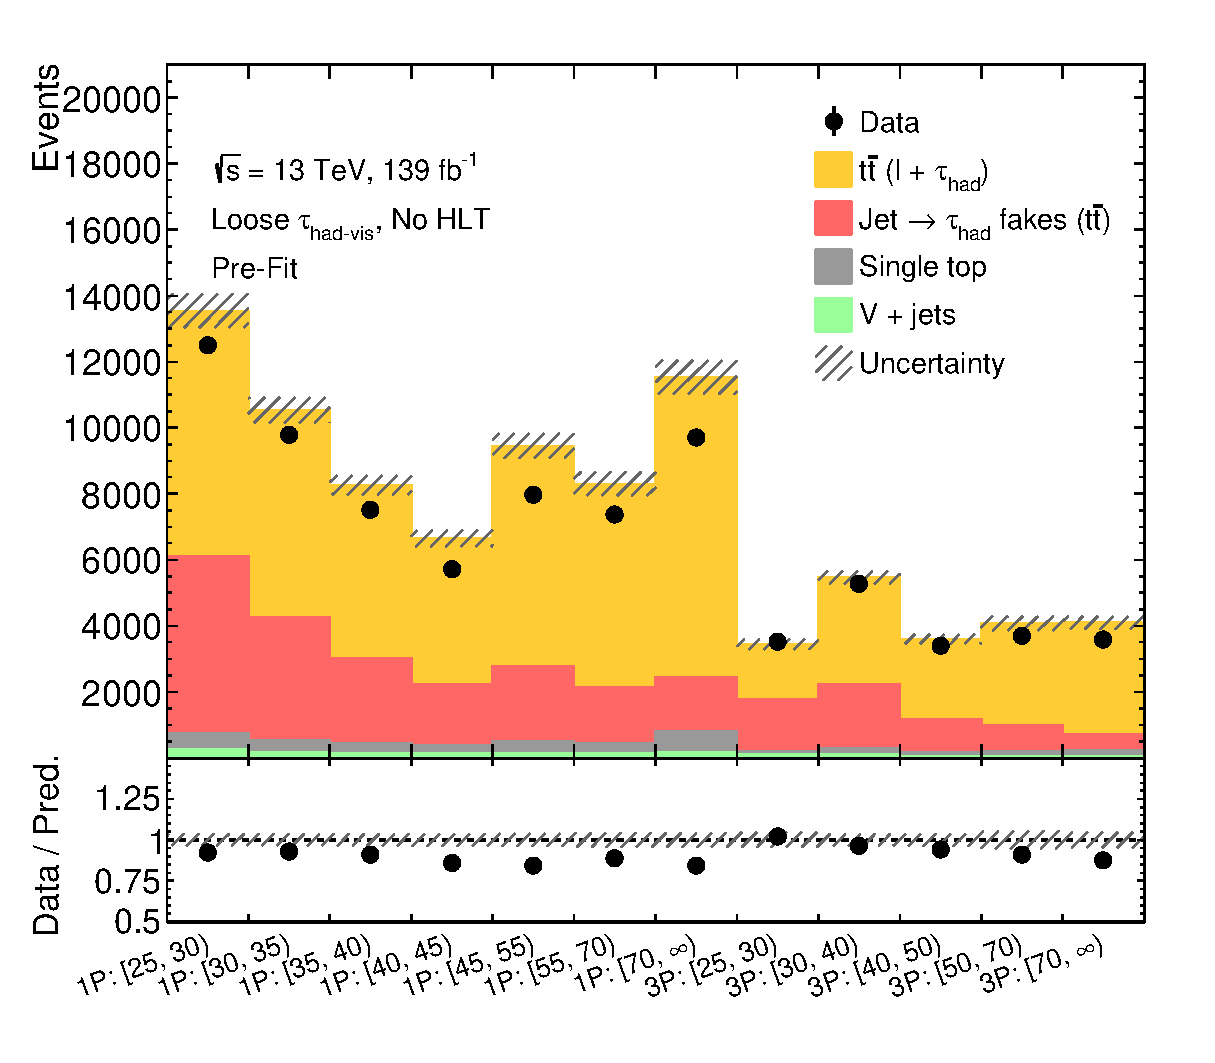
\includegraphics[width=\textwidth]{ttbarSF/Summary_offl}
    \caption{No HLT identification}
  \end{subfigure}%
  \begin{subfigure}{.5\textwidth}
    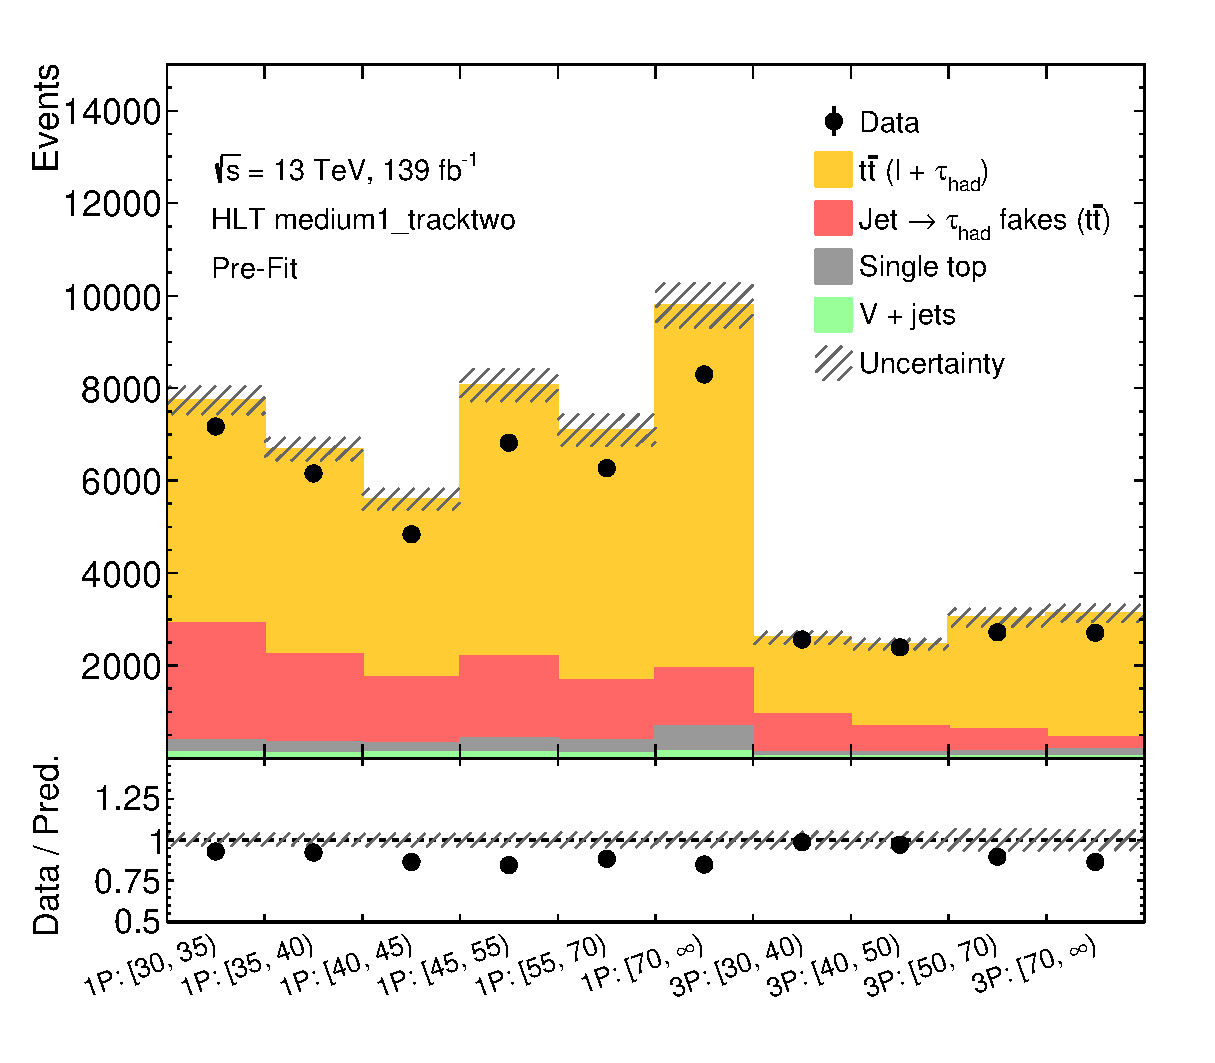
\includegraphics[width=\textwidth]{ttbarSF/Summary_tau25}
    \caption{With HLT identification}
  \end{subfigure}

  \caption{Summary of fit regions. Explain nomenclature on x-axis.}
\end{figure}


\begin{figure}[htbp]
  \centering

  \begin{subfigure}{.5\textwidth}
    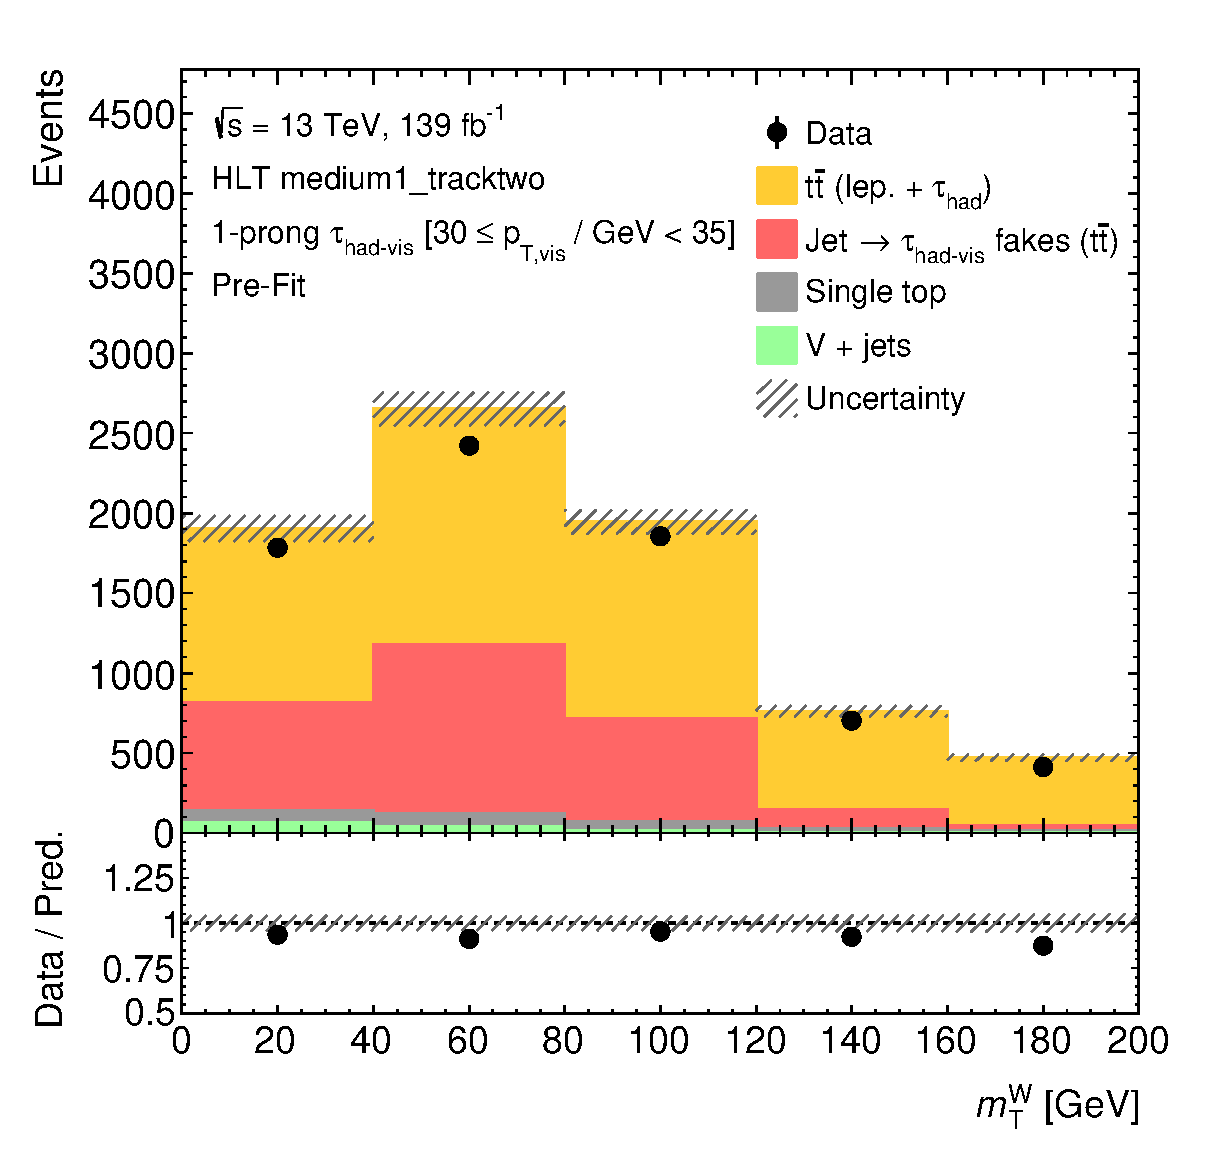
\includegraphics[width=\textwidth]{ttbarSF/tau25/TauPt3035_1P}
    \caption{a}
  \end{subfigure}%
  \begin{subfigure}{.5\textwidth}
    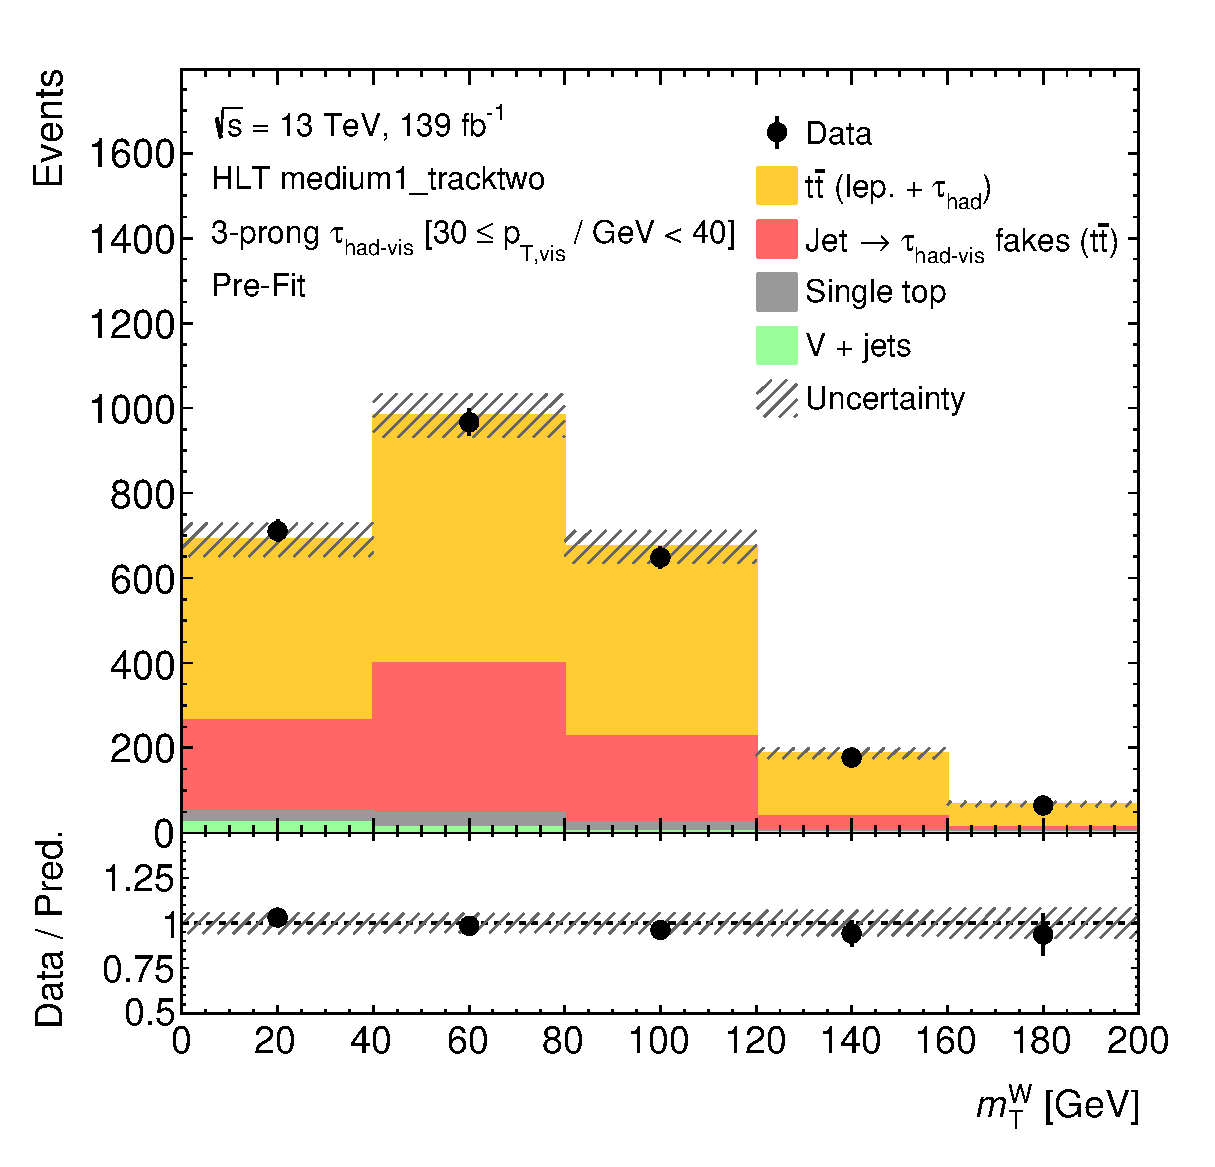
\includegraphics[width=\textwidth]{ttbarSF/tau25/TauPt3040_3P}
    \caption{b}
  \end{subfigure}

  \caption{Two examples of \mTW distributions}
\end{figure}




%%% Local Variables:
%%% mode: latex
%%% TeX-master: "../../phd_thesis"
%%% End:
